\documentclass{article}
\usepackage[utf8]{inputenc}
\usepackage[russian]{babel}
\usepackage{amsmath}
\usepackage{graphicx}
\usepackage{hyperref}

\title{Отчет по лабораторной работе \\ Реализация методов градиентного спуска}
\author{ \it Д. Чупров, Д. Серов, М. Боин, Н. Галимуллин }
\date{\today}

\begin{document}

\maketitle

% Формально не требуют, мб убрать

\begin{center}
{ \sc 0. Введение }
\end{center}

В данной работе реализованы различные стратегии градиентного спуска для оптимизации функций. Основное внимание уделено методам выбора шага обучения, включая постоянный шаг, адаптивные стратегии и методы, основанные на условиях Вольфе и Армихо. Реализация выполнена на Python с использованием библиотек NumPy и SciPy. В качестве тестовых функций использованы квадратичные функции произвольной размерности.

% [Описание методов] В начале отчёта опишите используемые методы. В
% описании метода укажите, это реализованный Вами или библиотечный метод,
% из какой библиотеки он взят, или какую библиотеку использует внутри
% реализации, если использует. При наличии, указывайте важные особенности
% Вашей реализации метода, они могут быть алгоритмические (например,
% имеющиеся hyperпараметры), так и технические (например, использование
% мемоизации в алгоритме).

\begin{center}
{ \sc 1. Описание методов }
\end{center}


Нами был реализован метод градиентного спуска со следующими алгоритмами подбора шага

        % AlgoData("Constant ", constant(0.3)),
        % AlgoData("Exponential Decay", exponential_decay(0.01)),
        % AlgoData("Polynomial Decay", polynomial_decay(0.5, 1)),

        % AlgoData("Armijo", armijo_rule),
        % AlgoData("Wolfe Rule", wolfe_rule),

\begin{enumerate}
    \item Постоянный шаг (сonstant)

    \item Экпоненциальное затухание (exponential decay)

    \item Полинимиальное затухание (polynomial decay)

    \item Правило Армихо (Armijo rule)

    \item Условие Вольфе (Wolfe rule)
\end{enumerate}

        % AlgoData("SciPy Armijo", scipy_armijo),
        % AlgoData("SciPy Wolfe", scipy_wolfe)

Кроме этого, для сравнения резульатов работы мы использовали следующие методы

\begin{enumerate}
    \item Правило Армихо (SciPy Armijo rule)

    \item Условие Вольфе (SciPy Wolfe rule)
\end{enumerate}

реализованные в библиотеке SciPy.optimize.\\[2mm]


Из особенностей реализации можно выделить то, что в Armijo rule и Wolfe rule так же накладывается ограничение на количество выполняемых итераций.

\vspace{2mm}

Для каждой из рассматриваемых функций дополнительно проведён анализ их геометрических свойств, влияющих на эффективность методов оптимизации. В частности, оценивается \textbf{число обусловленности} $\kappa$ — отношение максимального к минимальному собственному значению матрицы Гессе в заданной точке:
\[
\kappa = \frac{\lambda_{\max}}{\lambda_{\min}}.
\]

Малое значение $\kappa$ указывает на «сферическую» форму поверхности, благоприятную для градиентного спуска. Значения $\kappa \approx 1$ считаются \textit{оптимальными}, при этом градиент указывает практически в сторону минимума, и метод сходится быстро. Напротив, большие значения $\kappa$ (например, $10^3$ и выше) указывают на «вытянутую» форму поверхности, при которой градиентный спуск может сильно замедляться и колебаться.

Для наглядной визуализации используется преобразование:
\[
\log(1 + \kappa),
\]
которое позволяет отобразить широкий диапазон обусловленностей на одной цветовой шкале. Значения $\log(1 + \kappa) < 3$ считаются хорошими, в то время как $\log(1 + \kappa) > 7$ свидетельствуют о плохой обусловленности и потенциальной численной нестабильности.

На соответствующих картах обусловленности, приведённых для каждой функции, яркие области указывают на зоны высокой сложности для оптимизации. Это помогает объяснить разницу в поведении различных стратегий градиентного спуска.

\vspace{3mm}

% Это решение обсу


\begin{center}
    {\sc 2. Функции для иследования}
\end{center}

Для иллюстрации работы объявленных методов мы рассмотрим результаты программы на следующих функциях

% [Описание результатов]
% В результатах работы метода должна быть следующая информация:
% - объект исследования (функция) к которой применяется метод,

\begin{enumerate}
    0. { \bf Квадратичная функция }
    $$ f(x, y) = x^2 + y^2 $$.
\end{enumerate}

\begin{center}
    \includegraphics[scale=0.7]{grphcs/qf.png}

    { \it Карта обусловленности}
\end{center}

Различные методы спуска со стартовой точкой (-3, 5) и соответствующими начальными значениями гиперпараметров, указанными в таблице, дают следующие результаты

\begin{center}
{ \scriptsize
\begin{verbatim}
+-------------------+------------------------+------------------------+------------------------+----------------+-------+
|       Method      |         Params         |           x1           |           x2           | Gradient count | Steps |
+-------------------+------------------------+------------------------+------------------------+----------------+-------+
|     Wolfe Rule    | a=0.5, c1=1e-4, c2=0.3 |          0.0           |          0.0           |       8        |   2   |
|    SciPy Armijo   |           !            |          0.0           |          0.0           |       4        |   2   |
|  Polynomial Decay |       a=0.5, b=1       |          0.0           |          0.0           |       3        |   3   |
|    SciPy Wolfe    |           !            | -3.918306651365114e-20 | -2.350550309950183e-20 |       12       |   3   |
| Exponential Decay |         l=0.01         | 4.232351008428978e-05  | -7.053917277888955e-05 |       7        |   7   |
|      Constant     |         l=0.3          | -5.03316473035816e-05  | 8.388607980564544e-05  |       12       |   12  |
|       Armijo      |  a=0.9, q=0.5, c=0.5   | 0.00020416942289377374 | -0.0003402823706067735 |       43       |   43  |
|      Constant     |        l=0.003         | -0.007259254732917599  |  0.012098757890067957  |      1001      |  1001 |
+-------------------+------------------------+------------------------+------------------------+----------------+-------+
\end{verbatim}
}
{ \it Результаты спуска при начальной точке (-3, 5)}
\end{center}

Траектория спуска в соответствующих методах с начальными данными, привденными в таблице



\begin{center}
    \includegraphics[scale=0.7]{grphcs/Функции/Функция квадратичная/[-3.0, 5.0]/armijo_rule_gen(α=0.9, q=0.5, c=0.5)/2a3d.png}

    { \it Armijo}
\end{center}

\begin{center}
    \includegraphics[scale=0.7]{grphcs/Функции/Функция квадратичная/[-3.0, 5.0]/constant(λ=0.3)/2a3d.png}

    { \it Const}
\end{center}

\begin{center}
    \includegraphics[scale=0.7]{grphcs/Функции/Функция квадратичная/[-3.0, 5.0]/exponential_decay(λ=0.01)/2a3d.png}

    { \it Exponential decay}
\end{center}

\begin{center}
    \includegraphics[scale=0.7]{grphcs/Функции/Функция квадратичная/[-3.0, 5.0]/polynomial_decay(α=0.5, β=1)/2a2d.png}

    { \it Polynomial decay}
\end{center}

\begin{center}
    \includegraphics[scale=0.7]{grphcs/Функции/Функция квадратичная/[-3.0, 5.0]/wolfe_rule_gen(α=0.5, c1=1e-4, c2=0.3)/2a3d.png}

    { \it Wolfe}
\end{center}

\begin{enumerate}
    1. { \bf Функция Розенброка }
    $$ 0.1(1 - x)^2 + 0.1(y - x^2)^2 $$.
\end{enumerate}

\begin{center}
    \includegraphics[scale=0.7]{grphcs/rf.png}

    { \it Карта обусловленности}
\end{center}

% TODO:написать как сортим

Различные методы спуска со стартовой точкой (-1, 5) и соответствующими начальными значениями гиперпараметров, указанными в таблице, дают следующие результаты

\begin{center}
{ \scriptsize
\begin{verbatim}
+-------------------+------------------------+---------------------+--------------------+----------------+-------+
|       Method      |         Params         |          x1         |         x2         | Gradient count | Steps |
+-------------------+------------------------+---------------------+--------------------+----------------+-------+
|    SciPy Wolfe    |           !            |  0.9909960511304885 | 0.9801281016742087 |      160       |   46  |
|     Wolfe Rule    | a=0.5, c1=1e-4, c2=0.3 |  0.9933723089299055 | 0.9802210215506664 |      421       |   34  |
|       Armijo      |  a=0.9, q=0.5, c=0.5   |  0.9895221947688713 | 0.9747806373552036 |      127       |  127  |
|    SciPy Armijo   |           !            |  0.9892623061755571 | 0.9741570716870834 |      466       |  233  |
|      Constant     |         l=0.3          |  0.989093539246785  | 0.9737521858155559 |      388       |  388  |
| Exponential Decay |         l=0.01         |  -1.051806150400987 | 1.8958788742086938 |      1001      |  1001 |
|  Polynomial Decay |       a=0.5, b=1       | -1.6042352904667143 | 3.311470951930458  |      1001      |  1001 |
|      Constant     |        l=0.003         | -1.8697625414966101 | 4.2121694918899815 |      1001      |  1001 |
+-------------------+------------------------+---------------------+--------------------+----------------+-------+
\end{verbatim}
}
{ \it Результаты спуска при начальной точке (-1, 5)}
\end{center}

Траектория спуска в соответствующих методах с начальными данными, привденными в таблице

\begin{center}
    \includegraphics[scale=0.09]{grphcs/ros/(-1,5)armijo.png}

    { \it Armijo}
\end{center}

\begin{center}
    \includegraphics[scale=0.09]{grphcs/ros/(-1,5)const.png}

    { \it Const}
\end{center}

\begin{center}
    \includegraphics[scale=0.09]{grphcs/ros/(-1,5)wolfe.png}

    { \it Wolfe}
\end{center}

Различные методы спуска со стартовой точкой (0, 5) и соответствующими начальными значениями, указанными в таблице, дают следующие результаты

\newpage

\begin{center}
{ \scriptsize
\begin{verbatim}
+-------------------+------------------------+--------------------+--------------------+----------------+-------+
|       Method      |         Params         |         x1         |         x2         | Gradient count | Steps |
+-------------------+------------------------+--------------------+--------------------+----------------+-------+
|     Wolfe Rule    | a=0.5, c1=1e-4, c2=0.3 | 1.0071572817303238 | 1.020432090143632  |      236       |   17  |
|    SciPy Wolfe    |           !            | 1.0092345772827138 | 1.022234265176168  |      191       |   57  |
|       Armijo      |  a=0.9, q=0.5, c=0.5   | 1.0108045683605715 | 1.0261662061936638 |      156       |  156  |
|    SciPy Armijo   |           !            | 1.0108808227342037 | 1.0263514935232094 |      610       |  305  |
|      Constant     |         l=0.3          | 1.0110540145030602 | 1.0267722964998618 |      522       |  522  |
| Exponential Decay |         l=0.01         | 1.4856640225153208 | 2.355064255531157  |      1001      |  1001 |
|  Polynomial Decay |       a=0.5, b=1       | 1.6015796440743384 | 2.737071834811873  |      1001      |  1001 |
|      Constant     |        l=0.003         | 1.7662528067690704 | 3.418149817140798  |      1001      |  1001 |
+-------------------+------------------------+--------------------+--------------------+----------------+-------+
\end{verbatim}
}
{ \it Результаты спуска при начальной точке (0, 5)}
\end{center}

Соответствующие графики выбора траектории

\begin{center}
    \includegraphics[scale=0.09]{grphcs/ros/(0,5)armijo.png}

    { \it Armijo}
\end{center}

\begin{center}
    \includegraphics[scale=0.09]{grphcs/ros/(0,5)const.png}

    { \it Const}
\end{center}

\begin{center}
    \includegraphics[scale=0.09]{grphcs/ros/(0,5)wolfe.png}

    { \it Wolfe}
\end{center}

\newpage

\begin{enumerate}
    2. { \bf Функция Химмельблау - мультимодальная функция. }
    $$ f(x, y) = (x^2 + y - 11)^2 + (x + y^2 - 7)^2 $$.
\end{enumerate}

\begin{center}
    \includegraphics[scale=0.7]{grphcs/Функции/Карты обусловленности/HimmelblauMap.png}

    { \it Карта обусловленности}
\end{center}

Различные методы спуска со стартовой точкой (-4, -4) и соответствующими начальными значениями гиперпараметров, указанными в таблице, дают следующие результаты

\begin{center}
{ \scriptsize
\begin{verbatim}
+-------------------+------------------------+---------------------+---------------------+----------------+-------+
|       Method      |         Params         |          x1         |          x2         | Gradient count | Steps |
+-------------------+------------------------+---------------------+---------------------+----------------+-------+
|      Constant     |         l=0.3          |         nan         |         nan         |      1001      |  1001 |
|      Constant     |        l=0.003         |  -3.77931492713788  | -3.2831935273118904 |       46       |   46  |
| Exponential Decay |         l=0.01         |         nan         |         nan         |      1001      |  1001 |
|  Polynomial Decay |       a=0.5, b=1       |         nan         |         nan         |      1001      |  1001 |
|    SciPy Armijo   |           !            |  -3.77931022596459  | -3.2831872567553106 |       32       |   16  |
|    SciPy Wolfe    |           !            |  -3.779309030476698 |  -3.283185080081175 |       43       |   10  |
|     Wolfe Rule    | a=0.5, c1=1e-4, c2=0.3 | -3.7793132279563677 | -3.2831838001612166 |      103       |   11  |
|       Armijo      |  a=0.9, q=0.5, c=0.5   |  -3.782598582582645 | -3.2811377511278184 |      1001      |  1001 |
+-------------------+------------------------+---------------------+---------------------+----------------+-------+
\end{verbatim}
}
{ \it Результаты спуска при начальной точке (-4, -4)}
\end{center}

Траектория спуска в соответствующих методах с начальными данными, привденными в таблице

\begin{center}
    \includegraphics[scale=0.09]{grphcs/him/(-4,-4)armijo3d.png}

    { \it Armijo}
\end{center}

\begin{center}
    \includegraphics[scale=0.09]{grphcs/him/(-4,-4)const3d.png}

    { \it Const}
\end{center}

\begin{center}
    \includegraphics[scale=0.7]{grphcs/Функции/Функция Химмельбау/[-4.0, -4.0]/wolfe_rule_gen(α=0.5, c1=1e-4, c2=0.3)/2a2d.png}

    { \it Wolfe}
\end{center}


Различные методы спуска со стартовой точкой (0, -1) и соответствующими начальными значениями, указанными в таблице, дают следующие результаты

\newpage

\begin{center}
{ \scriptsize
\begin{verbatim}
+-------------------+------------------------+---------------------+---------------------+----------------+-------+
|       Method      |         Params         |          x1         |          x2         | Gradient count | Steps |
+-------------------+------------------------+---------------------+---------------------+----------------+-------+
|      Constant     |         L=0.3          |         nan         |         nan         |      1001      |  1001 |
|      Constant     |        l=0.003         |  3.5844256385929363 | -1.8480969256871265 |      151       |  151  |
| Exponential Decay |         l=0.01         |         nan         |         nan         |      1001      |  1001 |
|  Polynomial Decay |       a=0.5, b=1       |         nan         |         nan         |      1001      |  1001 |
|    SciPy Armijo   |           !            |  3.5844283213180934 | -1.8481263451027305 |      236       |  118  |
|     Wolfe Rule    | a=0.5, c1=1e-4, c2=0.3 | -3.7793132368280022 | -3.2831837261692227 |      126       |   14  |
|    SciPy Wolfe    |           !            |  3.5844261682851597 | -1.8481173445474242 |       65       |   15  |
|       Armijo      |  a=0.9, q=0.5, c=0.5   |  3.5992933786358363 |  -1.846765158117622 |      1001      |  1001 |
+-------------------+------------------------+---------------------+---------------------+----------------+-------+
\end{verbatim}
}
{ \it Результаты спуска при начальной точке (0, -1)}
\end{center}

Соответствующие графики выбора траектории

\begin{center}
    \includegraphics[scale=0.7]{grphcs/Функции/Функция Химмельбау/[0.0, -1.0]/armijo_rule_gen(α=0.9, q=0.5, c=0.5)/2a3d.png}

    { \it Armijo}
\end{center}

\begin{center}
    \includegraphics[scale=0.7]{grphcs/Функции/Функция Химмельбау/[0.0, -1.0]/constant(λ=0.003)/2a3d.png}

    { \it Const}
\end{center}

\begin{center}
    \includegraphics[scale=0.7]{grphcs/Функции/Функция Химмельбау/[0.0, -1.0]/wolfe_rule_gen(α=0.5, c1=1e-4, c2=0.3)/2a2d.png}

    { \it Wolfe}
\end{center}

В силу мультимодальности функции при разных стартовых значениях получаются разные минимумы, причем не обязательно, что функция сойдется к ближайшему минимуму. Например, в реализации метода спуска с правилом Вольфе, мы видим, что шаг спуска прыгнул настолько далеко, что попал в противоположный минимум.

\newpage

    3. { \bf Полусфера. }
    $$ f(x, y) = 10 - \sqrt{100 - x^2 - y^2}$$.


    \begin{center}
    \includegraphics[scale=0.7]{grphcs/sf.png}

    { \it Карта обусловленности}
\end{center}

Различные методы спуска со стартовой точкой (-3, 2) и соответствующими начальными значениями гиперпараметров, указанными в таблице, дают следующие результаты

\begin{center}
{ \scriptsize
\begin{verbatim}
+-------------------+------------------------+------------------------+-----------------------+----------------+-------+
|       Method      |         Params         |           x1           |           x2          | Gradient count | Steps |
+-------------------+------------------------+------------------------+-----------------------+----------------+-------+
|     Wolfe Rule    | a=0.5, c1=1e-4, c2=0.3 | -0.0007798466831445694 | 0.0005178609862923622 |      100       |   4   |
|    SciPy Wolfe    |           !            | -0.004064384049968672  |  0.002709090668526537 |      124       |   40  |
|       Armijo      |  a=0.9, q=0.5, c=0.5   | -0.006905007700233843  |  0.00460331990840529  |       64       |   64  |
|    SciPy Armijo   |           !            | -0.007542452912672193  |  0.00502861643930419  |      232       |  116  |
|      Constant     |         l=0.3          |  -0.00786652354721598  |  0.005244551615252768 |      194       |  194  |
| Exponential Decay |         l=0.01         |  -0.5489211054395599   |  0.36594754094491266  |      1001      |  1001 |
|  Polynomial Decay |       a=0.5, b=1       |  -1.3679405987438222   |   0.9119604260644844  |      1001      |  1001 |
|      Constant     |        l=0.003         |   -2.187229196282272   |   1.4581527785622328  |      1001      |  1001 |
+-------------------+------------------------+------------------------+-----------------------+----------------+-------+
\end{verbatim}
}
{ \it Результаты спуска при начальной точке (-3, 2)}
\end{center}


Траектория спуска в соответствующих методах с начальными данными, привденными в таблице

\begin{center}
    \includegraphics[scale=0.09]{grphcs/s/exp.png}

    { \it Exponential Decay}
    { \it Из-за высокой скорости затухания экспоненциального выбора шага, число итераций сходимости велико и сильно превышает установленный лимит в количество шагов. Поэтому мы видим, что метод градиентного спуска, основанный на экспоненциальной стратегии выборе шага, а также на полиномиальной стратегии по тем же причинам дают неверные ответы}
\end{center}

\begin{center}
    \includegraphics[scale=0.09]{grphcs/s/const(0.3).png}

    { \it Const}
\end{center}

\begin{center}
    \includegraphics[scale=0.09]{grphcs/s/wolfe.png}

    { \it Wolfe}
\end{center}



    4. { \bf Квадратичная функция с зашумлением. }
    $$ f(x, y) = x^2+y^2+ 0.01 * np.random.randn()$$.

Различные методы спуска со стартовой точкой (-2,2) и соответствующими начальными значениями гиперпараметров, указанными в таблице, дают следующие результаты


\begin{center}
{ \scriptsize
\begin{verbatim}

+-------------------+------------------------+-----------------------+---------------------+----------------+-------+
|       Method      |         Params         |           x1          |          x2         | Gradient count | Steps |
+-------------------+------------------------+-----------------------+---------------------+----------------+-------+
|       Armijo      |  a=0.9, q=0.5, c=0.5   |   0.2707812341750599  | 0.09458333070860024 |      1001      |  1001 |
|  Polynomial Decay |       a=0.5, b=1       | -0.039241003494682576 | -0.3701033435165779 |      163       |  163  |
| Exponential Decay |         l=0.01         |   0.4262633939718083  | -0.2916166637349709 |      244       |  244  |
|     Wolfe Rule    | a=0.5, c1=1e-4, c2=0.3 |  -0.34855046739582396 |  0.4085727839652793 |      414       |   43  |
|    SciPy Wolfe    |           !            |  -0.8155710283010043  | -0.9163512900446878 |       37       |   8   |
|    SciPy Armijo   |           !            |   -1.279405451678135  | 0.25152011089535525 |       16       |   8   |
|      Constant     |         l=0.3          |  0.17779825414640382  |  1.0134968516034732 |      1001      |  1001 |
|      Constant     |        l=0.003         |  -1.8965436532837217  |  1.8081264978318343 |       22       |   22  |
+-------------------+------------------------+-----------------------+---------------------+----------------+-------+
\end{verbatim}
}
{ \it Результаты спуска при начальной точке (-2,-2)

Все методы работают достаточно неплохо кроме константного недостаточной длиной шага}
\end{center}

Траектория спуска в соответствующих методах с начальными данными, привденными в таблице

\begin{center}
    \includegraphics[scale=0.7]{grphcs/Функции/Функция квадратичная зашумленная/шум с амплитудой 1/armijo_rule_gen(α=0.9, q=0.5, c=0.5)/2a3d.png}

    { \it Armijo}
\end{center}

\begin{center}
    \includegraphics[scale=0.7]{grphcs/Функции/Функция квадратичная зашумленная/шум с амплитудой 1/constant(λ=0.3)/2a3d.png}

    { \it Const}
\end{center}

\begin{center}
    \includegraphics[scale=0.7]{grphcs/Функции/Функция квадратичная зашумленная/шум с амплитудой 1/polynomial_decay(α=0.5, β=1)/2a3d.png}

    { \it Polynomial decay}
\end{center}

\begin{center}
    \includegraphics[scale=0.7]{grphcs/Функции/Функция квадратичная зашумленная/шум с амплитудой 1/wolfe_rule_gen(α=0.5, c1=1e-4, c2=0.3)/2a3d.png}

    { \it Wolfe}
\end{center}

\begin{center}
    {\sc 4. Вывод}
\end{center}

\section*{Вывод}
В ходе лабораторной работы были реализованы и протестированы различные стратегии выбора шага в алгоритме градиентного спуска, а именно: метод постоянного шага, экспоненциальное и полиномиальное затухание, а также адаптивные методы, основанные на правилах Армихо и Вольфе (включая реализации из библиотеки SciPy). Проведённый анализ экспериментов на ряде тестовых функций (квадратичной, функции Розенброка, функции Химмельблау, полусферы и квадратичной функции с зашумлением) позволяет сделать следующие выводы:

\begin{enumerate}
    \item \textbf{Адаптивные методы (Армихо и Вольфе):} \\
    Эти стратегии продемонстрировали высокую точность в нахождении минимума, автоматически адаптируя шаг обучения к характеристикам целевой функции. Особенно на сложных и плохо обусловленных функциях (например, функция Розенброка и Химмельблау), методы на основе условий Армихо и Вольфе обеспечивают приближение к оптимуму с меньшей погрешностью. Хотя количество вычислений градиента может быть больше, они оправдывают себя при необходимости достижения высокой точности.

    \item \textbf{Стратегии с экспоненциальным и полиномиальным затуханием, а также постоянный шаг:} \\
    На простых, «сферических» функциях, таких как квадратичная, данные методы показывают конкурентные результаты за счёт меньшего количества итераций и вычислений градиента. Экспериментальные данные указывают на более быструю сходимость этих стратегий, что особенно важно при ограниченных вычислительных ресурсах.

    \item \textbf{Поведение на зашумлённых функциях:} \\
    Наблюдения показывают, что экспоненциальное и полиномиальное затухание, которые хорошо работают на стандартных квадратичных функциях, демонстрируют неплохую стабильность и при добавлении шума. Это может указывать на то, что данные стратегии способны адекватно учитывать случайные колебания значений простых функций, таких как квадратичная или сферическая. Однако стоит отметить, что на более сложных функциях, особенно с малой кривизной, как, например, функция Розенберка, присутствие шума может значительно усложнить поиск минимума.

    \item \textbf{Выбор метода в зависимости от вычислительных затрат:} \\
    Если вычисление градиента происходит достаточно быстро и требуется высокая точность, оптимальным выбором являются методы с условиями Армихо и Вольфе. Однако при значительных вычислительных затратах или если функция относительно проста, разумно рассмотреть стратегии планирования (расписания) шага, позволяющие снизить число вычислений за счёт использования фиксированных или медленно затухающихся параметров.

    \item \textbf{Гибкость реализации:} \\
    Разработанная система позволяет легко переключаться между различными стратегиями и настраивать параметры алгоритма, что даёт возможность адаптировать метод градиентного спуска под особенности решаемой задачи. Такой подход обеспечивает баланс между точностью нахождения минимума и вычислительной эффективностью.
\end{enumerate}

Таким образом, результаты работы подтверждают, что оптимальный выбор стратегии шага существенно зависит от геометрических свойств целевой функции и вычислительных ограничений. При грамотном подборе метода можно добиться как высокой точности, так и экономии вычислительных ресурсов, что является важным аспектом при решении реальных задач оптимизации.

\end{document}
